\section{Introduction}
\label{s:intro}

The Department of Energy (DOE) Nuclear Energy (NE) Center of Excellence for Thermal-fluid applications in Nuclear Energy (COE) \cite{shaver2019initial} inaugurated in April 2018 researches novel solution strategies to historically challenging issues involving fluid flow in nuclear reactors. These include issues that still plague the current fleet of deployed Light-Water Reactors (LWRs) and predict various fluid flow and fluid-related phenomena within advanced reactor technologies. Advanced-reactors studied include Small Modular Reactor (SMR) concepts, micro-reactors, and Advanced Reactor Concepts (ARC), utilizing coolants such as liquid metal, chloride, and fluoride salts, or gas, for accident-tolerant reactors. These new solution strategies and algorithms are implemented using modern software design methodology, best software quality practices, and then delivering validated NQA-1 level software to the nuclear power community.

Our advanced thermal-fluids research and development approach synergistically combines three natural, overlapping, length and time scales in a hierarchal multi-scale approach to avoid the temptation and
pitfalls of attempting to develop a single solve-all algorithm for physical fluid flow problems that will span nine orders of magnitude in spatial and temporal scales. A more tractable approach is grouping physics with similar multi-scale requirements into a common algorithm, developing separate software applications to address the separate scales, and coupling the appropriate applications. This multi-scale modeling and simulation template has proven to be highly successful in the Nuclear Energy Advanced Modeling and Simulation (NEAMS) program to simulate nuclear material evolution under irradiation \cite{tonks2013multiscale}. The three overlapping thermal-hydraulic scales are defined across all reactor concepts as:
\begin{itemize}
    \item \textbf{Lower Length Scale.} The Lower Length Scale will resolve high-resolution physics
    associated with single and multi-phase, highly turbulent conjugate heat transfer (CHT) with highly
    resolved thermal boundary layers (heat flux).
    \item \textbf{Engineering Length scale.} The Engineering Length Scale will integrate coarse mesh approaches
    for homogenized multi-dimensional CHT, such as those found in gas-cooled pebble-bed reactors, or three-dimensional sub-channel capabilities tightly coupled to nuclear fuels performance.
    \item \textbf{System Scale.} System Scale analysis for nuclear reactors is composed of one-dimensional fluid flow
    pipe networks and zero-dimensional system components. These classes of algorithms and corresponding approaches are treated as reduced-order models (ROM) of the more complex scales and allow for more efficient calculations. These reduced-order systems rely heavily on empirical correlations or models, as many of the flow features and phenomena are no longer resolved.
\end{itemize}

To demonstrate the multi-scale philosophy of the center, we focus first on Flouride Cooled High-Temperature Reactors (FHRs) \cite{forsberg2015fluoride}, and in particular on Berkeley's PB-FHR design Mark-I design \cite{cisneros2014technical}. The Fluoride salt cooled High-temperature Reactor (FHR) is a class of advanced nuclear reactors that combines the robust coated particle fuel form from high-temperature gas-cooled reactors, direct reactor auxiliary cooling system (DRACS) passive decay removal of liquid metal fast reactors, and the transparent, high volumetric heat capacitance liquid fluoride salt working fluids (e.g., FLiBe)) from molten salt reactors. This combination of fuel and coolant enables FHRs to operate in a high-temperature, low-pressure design space that has beneficial safety and economic implications. In 2012, UC Berkeley was charged with developing a pre-conceptual design of a commercial prototype FHR --- the Pebble Bed Fluoride Salt Cooled High-Temperature Reactor (PB-FHR) \cite{cisneros2014technical}. The Mark 1 design of the PB-FHR (Mk1 PB-FHR) is a 236 MWt FLiBe cooled pebble-bed nuclear heat source that drives an open-air Brayton combined-cycle power conversion system. The PB-FHR's pebble bed consists of an enriched uranium fuel core surrounded by an inert graphite pebble region that shields the outer solid graphite region, core barrel, and reactor vessel. The fuel reaches an average burnup of 178000 MWt-d/MT. The Mk1 PB-FHR exhibits strong negative temperature reactivity feedback from the fuel, graphite moderator, and FLiBe coolant, but a small positive temperature reactivity feedback of the inner region and outer graphite pebble region. Pebble bed reactors are, in a sense, the poster child for the sort of analysis described above.

FHR pebble beds, in particular, are comprised of hundreds of thousands of pebbles, and a CFD-grade detailed description of the flow-field through these pebbles for an entire reactor core is not practical with current simulation technology. However, this manuscript will demonstrate a credible pathway toward a full-core, predictive, high-fidelity CFD capability for these reactors. For practical, fast-running, design-related purposes, porous media formulations have been employed in codes as THERMIX \cite{cleveland1986application} and AGREE \cite{seker2007multiphysics}. However, simple porous media approximations are often incapable of capturing the flow field's critical details, such as the wall channeling effect due to the change in porosity near the vessel walls.  Advanced formulations for the "engineering scale" can address these issues, but data from finer scale simulations is needed to build closure relationships for Pronghorn (\cite{novak2018pronghorn}, \cite{novak1}, \cite{novak2}), the platform of the COE. Finally, finer scale calculations are needed to establish local temperature peaking and fuel temperatures.

We note that fine-scale CFD simulations have been attempted before but not for large scale beds using Large Eddy simulation \cite{vanstaden2018}. This work represents the most extensive collection of large eddy simulations  (LES) ever attempted for random pebble beds.

One concept for an overall multiphysics strategy for FHR simulation is illustrated in Figure~\ref{f:fhr1}. SAM \cite{hu2017sam}, a systems analysis tool for advanced reactors with coolants in the liquid phase, drives the simulation of the engineering scale tools (Pronghorn and Rattlesnake/Mammoth \cite{wang1}). The lower length-scale tools can be run concurrently to provide dynamic closures for the engineering scale or offline to produce correlations (which would be more likely). The lower length-scale simulator may comprise neutronics (e.g., OpenMC \cite{romano2013openmc}), thermal-fluids (Nek5000-NekRS \cite{fischer2008}) and fuel performance (BISON \cite{hales2013triso}).

\begin{figure}[!h]
\centering
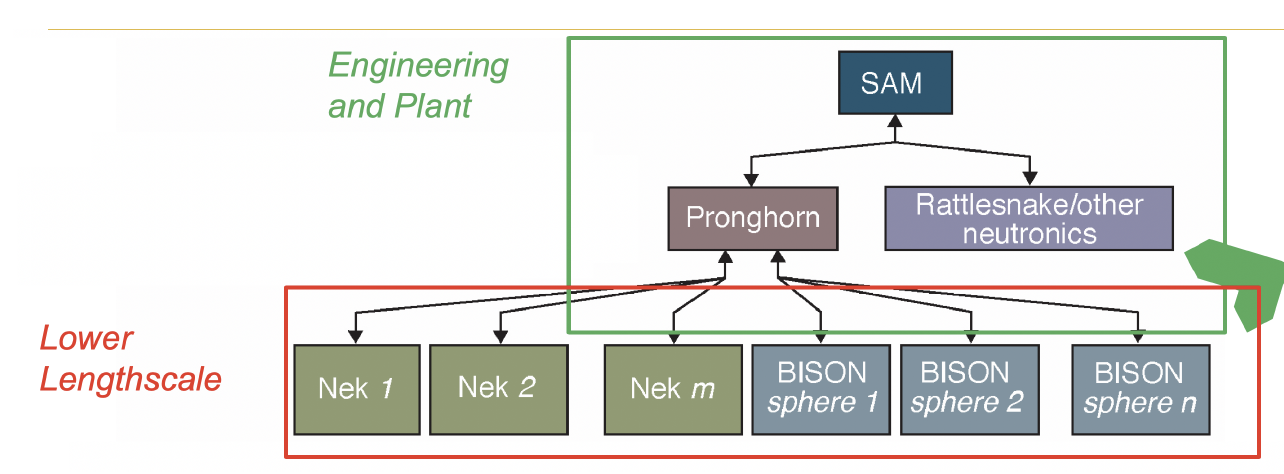
\includegraphics[clip=true,width=0.8\textwidth]{Figures/fhr_graph}
\caption{Diagram showing the multiscale structure of the COE simulator for FHRs.}
\label{f:fhr1}
\end{figure}

Cardinal, the tool developed here, is the COE tool for lower length-scale simulation for pebble beds. This new platform tightly couples all three physics and leverages advances in MOOSE \cite{gaston2009moose, permann2020moose}, such as the MultiApp system, and the concept of MOOSE-wrapped Apps \cite{gaston2015physics}. Moreover, it is designed from the ground-up to scale on massively parallel architectures and perform well on leadership-class supercomputing architectures. Initial efforts in the development of the Cardinal were presented in a recent report \cite{cardinal}. In this manuscript, we provide a significant advancement to the high fidelity modeling of FHR pebble beds. We also demonstrate a hybrid GPU-CPU model to leverage pre-exascale supercomputer architectures (i.e., Summit) and the potential of scaling to full-core simulations in the near future.

In this manuscript, we:
\begin{itemize}
\item Discuss the design and structure of Cardinal;
\item Discuss verification and validation;
\item Demonstrate the application of Cardinal to large scale pebble beds.
\end{itemize}

We emphasize the importance of the data generated with these high-fidelity conjugate heat transfer simulations of pebble beds. They represent an essential stepping stone for developing closure models for Pronghorn (e.g., models including the wall-channeling effects), and in general, a resource for confirmatory analysis of reduced-order models. While we do not focus here on using the data generated to extract closure relationships, this will be the subject of future publications.
